\section{Metodologia}
\label{sec:metodologia}

Esta seção descreve os dados disponíveis, como as FRFs foram obtidas e tratadas, como
as frequências naturais e os fatores de amortecimento foram identificados e como o
modelo da Seção~\ref{sec:intro} foi resolvido e ajustado. Todo o processamento foi
feito em Python, com NumPy, SciPy \cite{scipy2020} e Matplotlib com o estilo
SciencePlots \cite{scienceplots}. Os trechos principais aparecem ao longo do texto, e o
código completo está no Apêndice~\ref{ap:codigo}. O script
\texttt{gera\_resultados.py} gera todas as figuras e tabelas desta seção e da seguinte
a partir dos arquivos de dados, sem valores digitados à mão.

%=====================================================================
\subsection{Parâmetros da viga}
\label{sec:parametros}

A Tabela~\ref{tab:parametros} reúne os dados da viga \cite{roteiroLab1} e as
grandezas derivadas usadas no modelo. Dois pontos do roteiro merecem nota. Primeiro,
a massa $m_b = \SI{0.445}{\kilo\gram}$ listada na tabela de componentes não é a
massa da viga: com as dimensões e a massa específica informadas,
$\rho A L = \SI{0.632}{\kilo\gram}$. Ela é interpretada aqui como a massa
concentrada $m_{\mathrm{end}}$ da Figura~1 do roteiro, o que dá a razão de massas
$\mu = m/(\rho A L) = \num{0.705}$. Os ensaios, porém, foram feitos \emph{sem} essa
massa; ela só entra na comparação da Seção~\ref{sec:massa}. Segundo, usa-se
$\rho = \SI{8069.4}{\kilo\gram\per\cubic\meter}$, como no roteiro (o rascunho anterior
da análise usava $\num{8096.4}$, uma troca de dígitos que altera as frequências em
\SI{0.17}{\percent}).

\begin{table}[htbp]
    \centering
    \caption{Parâmetros da viga e da instrumentação.}
    \label{tab:parametros}
    \begin{tabular}{llr}
        \toprule
        Grandeza                                 & Símbolo                 & Valor                                      \\
        \midrule
        Largura                                  & $b$                     & \SI{26.0}{\milli\meter}                    \\
        Espessura                                & $h$                     & \SI{7.0}{\milli\meter}                     \\
        Comprimento livre                        & $L$                     & \SI{430}{\milli\meter}                     \\
        Módulo de elasticidade                   & $E$                     & \SI{210}{\giga\pascal}                     \\
        Massa específica                         & $\rho$                  & \SI{8069.4}{\kilo\gram\per\cubic\meter}    \\
        Rigidez à flexão                         & $EI = Ebh^3/12$         & \SI{156.07}{\newton\square\meter}          \\
        Massa por unidade de comprimento         & $\rho A$                & \SI{1.4686}{\kilo\gram\per\meter}          \\
        Massa da viga                            & $\rho A L$              & \SI{0.632}{\kilo\gram}                     \\
        Massa na ponta (não usada nos ensaios)   & $m$                     & \SI{0.445}{\kilo\gram}                     \\
        Razão de massas correspondente           & $\mu$                   & \num{0.705}                                \\
        Ponto de impacto (martelo)               & $x_i$                   & \SI{0.200}{\meter}                         \\
        Acelerômetro (martelo)                   & $x_e$                   & \SI{0.356}{\meter}                         \\
        Cabeça de impedância (\emph{shaker})     & $x_i = x_e$             & $L$                                        \\
        \bottomrule
    \end{tabular}
\end{table}

Os parâmetros ficam centralizados no módulo \texttt{parametros.py}, junto com a
conversão \eqref{eq:omega} entre $\lambda_r$ e a frequência em hertz,
$f_r = \omega_r/2\pi$ (Código~\ref{lst:parametros}).

\trecho[label={lst:parametros}]{parametros.py}{conversao}{[Conversão entre $\lambda_r$ e $f_r$]Conversão entre
    $\lambda_r$ e $f_r$ (\texttt{parametros.py}).}

%=====================================================================
\subsection{Ensaio com martelo de impacto}
\label{sec:met_martelo}

No ensaio com martelo a viga foi golpeada a \SI{0.200}{\meter} do engaste e a
aceleração foi medida a \SI{0.356}{\meter}, com o sistema Dewesoft a
\SI{5000}{\hertz}. Há dois arquivos: a FRF calculada pelo próprio Dewesoft
(estimadores $H_1$ e $H_2$ e coerência, média de três impactos) e a série temporal de
força e aceleração que a originou. A FRF exportada usa blocos de 2048 amostras, ou
seja, registros de \SI{0.41}{\second} e resolução $\Delta f = \SI{2.44}{\hertz}$. Essa
resolução é grosseira para o primeiro modo: a banda de meia potência de um modo com
$f_r \approx \SI{25}{\hertz}$ e $\zeta_r \approx \SI{2}{\percent}$ tem
$2\zeta_r f_r \approx \SI{1}{\hertz}$, menos que um intervalo de frequência. Além
disso, a resposta desse modo leva mais de \SI{1}{\second} para decair (constante de
tempo $1/(\zeta_1\omega_1) \approx \SI{0.26}{\second}$), de modo que um registro de
\SI{0.41}{\second} a trunca e espalha a energia do pico para as frequências vizinhas
(vazamento).

Por isso a FRF foi recalculada a partir da série temporal
(Figura~\ref{fig:martelo_serie}). Foram identificados três impactos, em
$t \approx \num{3.86}$; \num{9.70} e \SI{12.80}{\second}, com picos de força de
\num{12}, \num{34} e \SI{80}{\newton}. Os dois últimos têm um segundo contato
\SIrange{2.6}{3.0}{\milli\second} depois do primeiro (duplo impacto), visível no
detalhe da figura.
Para cada impacto tomou-se um registro de $T = \SI{3}{\second}$, começando
\SI{10}{\milli\second} antes do pico. A força foi zerada a partir de
\SI{20}{\milli\second} após o pico (janela de força), o que mantém o duplo impacto, que faz
parte da excitação aplicada, e elimina o ruído do canal de força no resto do registro.
A aceleração não recebeu janela: o detalhe inferior da Figura~\ref{fig:martelo_serie}
mostra que, nos três impactos, ela cai mais de três ordens de grandeza em
\SI{1.5}{\second}; no fim do registro de \SI{3}{\second}, seu valor eficaz é da ordem
do ruído medido antes do impacto (cerca de \SI{0.04}{\meter\per\second\squared}).
O registro contém, portanto, a resposta inteira, sem truncamento. Nessas condições, completar os registros com zeros até
$2^{17}$ pontos apenas interpola o espectro, com espaçamento de
\SI{0.038}{\hertz}, sem criar informação nova.

\begin{figure}[htbp]
    \centering
    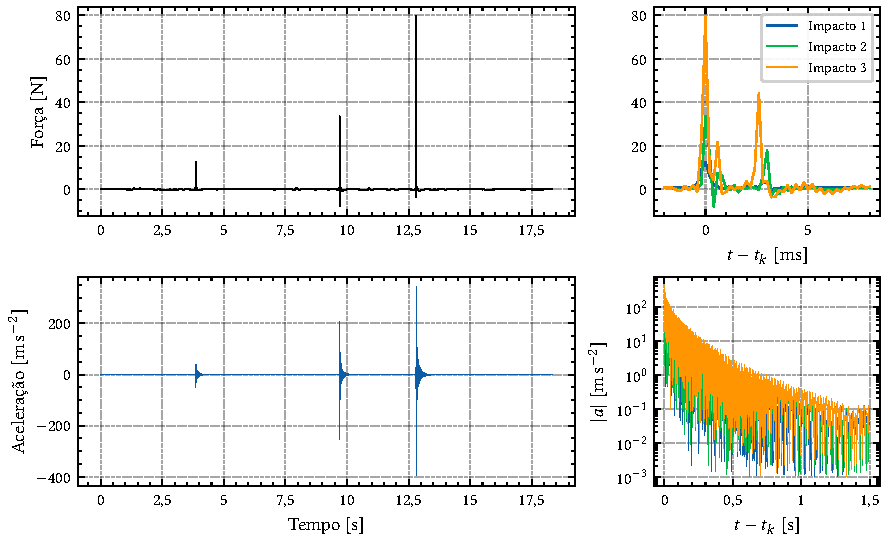
\includegraphics[width=\textwidth]{martelo_serie.pdf}
    \caption{Série temporal do ensaio com martelo. À esquerda, força e aceleração ao
        longo de todo o registro; à direita, detalhe dos pulsos de força (com o duplo
        impacto dos golpes 2 e 3) e decaimento de $|a(t)|$ após cada impacto $t_k$.}
    \label{fig:martelo_serie}
\end{figure}

Com os espectros $F_k(f)$ e $A_k(f)$ de força e aceleração de cada impacto $k$, os
autoespectros e o espectro cruzado são somados sobre os impactos,
\begin{equation}
    G_{ff} = \sum_k |F_k|^2, \qquad G_{aa} = \sum_k |A_k|^2, \qquad
    G_{fa} = \sum_k F_k^{*} A_k,
\end{equation}
e as FRFs e a coerência são \cite{ewins2000}
\begin{equation}
    H_1 = \frac{G_{fa}}{G_{ff}}, \qquad
    H_2 = \frac{G_{aa}}{G_{fa}^{*}}, \qquad
    \gamma^2 = \frac{|G_{fa}|^2}{G_{ff}\,G_{aa}} = \frac{H_1}{H_2}.
    \label{eq:estimadores}
\end{equation}
$H_1$ minimiza o efeito de ruído na resposta e $H_2$, o de ruído na força; a
coerência $\gamma^2 \le 1$ indica quanto da resposta é explicada linearmente pela
força medida. O Código~\ref{lst:frf_serie} implementa esse cálculo.

\trecho[label={lst:frf_serie}]{dados.py}{frf_serie}{[FRF do martelo a partir da série temporal]FRF do martelo a partir da série
    temporal (\texttt{dados.py}).}

Um último ajuste vale para os dois ensaios. Abaixo da primeira ressonância a viga
responde quase estaticamente: $w$ fica em fase com a força e $\ddot w = -\Omega^2 w$,
logo a acelerância deve ter fase $\pi$. Nos dois arquivos a fase medida nessa faixa é
próxima de zero, o que indica que o sentido positivo da força é oposto ao do
acelerômetro (o martelo e a célula de carga medem compressão). As FRFs medidas foram,
portanto, multiplicadas por $-1$ (constante \texttt{SINAL} em \texttt{dados.py}). Essa
correção é feita uma única vez e não usa o modelo; a concordância de sinal dos picos
com as formas modais, vista na Seção~\ref{sec:molas_res}, serve depois como
verificação independente.

%=====================================================================
\subsection{Ensaio com \emph{shaker}}
\label{sec:met_shaker}

No segundo ensaio a ponta livre foi ligada ao \emph{shaker} por uma haste
(\emph{stinger}) e uma cabeça de impedância, que mede a força transmitida e a aceleração
no mesmo ponto. O controlador Dactron fez uma varredura senoidal de \SIrange{5}{2000}{\hertz}
e exportou a transmissibilidade aceleração/força e a coerência em 512 frequências com
passo logarítmico de \SI{1.18}{\percent}. Trata-se, portanto, de uma acelerância
pontual em $x = L$, comparável a \eqref{eq:acelerancia} com $x_i = x_e = L$; a unidade
(\si{\meter\per\second\squared\per\newton}) foi confirmada pelo nível em baixa
frequência, da mesma ordem do previsto pelos modelos (Seção~\ref{sec:molas_res}); se
a razão estivesse em \si{g\per\newton}, apareceria um fator de \num{9.81}. O passo de \SI{1.18}{\percent} é da mesma ordem da banda
de meia potência dos modos pouco amortecidos ($2\zeta_r \approx
\SIrange{0.4}{1.2}{\percent}$), o que limita a precisão dos fatores de amortecimento
obtidos com esse ensaio.

%=====================================================================
\subsection{Identificação de frequências naturais e amortecimento}
\label{sec:met_identificacao}

Os picos de $|H|$ foram localizados pela proeminência em escala logarítmica: só são
aceitos picos que se destacam pelo menos meia década ($\approx 3\times$) dos vales
vizinhos, o que descarta oscilações de ruído. A frequência natural é a do máximo, e o
amortecimento vem do método da meia potência \cite{ewins2000}: sendo $f_1 < f_r < f_2$
as frequências em que $|H| = |H|_{\max}/\sqrt{2}$,
\begin{equation}
    \zeta_r = \frac{f_2 - f_1}{2 f_r}.
    \label{eq:meia_potencia}
\end{equation}
Como os pontos medidos raramente caem exatamente em $|H|_{\max}/\sqrt{2}$, cada
cruzamento é interpolado entre os dois pontos vizinhos, em $\log f$
(Código~\ref{lst:meia_potencia}). A rotina também conta quantos pontos medidos caem
dentro da banda $[f_1, f_2]$; com um ou dois pontos, a estimativa de $\zeta_r$ depende
mais da posição da grade de frequências do que do sistema.

\trecho[label={lst:meia_potencia}]{identificacao.py}{meia_potencia}{[Picos e método da meia potência]Picos e
    amortecimento pelo método da meia potência (\texttt{identificacao.py}).}

Os picos identificados são associados aos modos de flexão do modelo pela frequência
mais próxima, com tolerância de \SI{20}{\percent}; picos sem correspondente são
listados à parte.

%=====================================================================
\subsection{Solução numérica do modelo}
\label{sec:met_modelo}

As equações características \eqref{eq:car_engaste} e \eqref{eq:car_molas} crescem
como $\cosh\lambda$, que passa de $10^{8}$ para $\lambda > 20$. Para trabalhar com uma
função de ordem 1, ambas foram divididas por $\cosh\lambda$ e, no caso das molas,
também por $1 + \alpha_L\alpha_R > 0$; nenhuma das divisões altera as raízes. As
raízes são isoladas por uma varredura de sinal em $\lambda \in (0, 9\pi]$, com passo
$10^{-3}$, e refinadas pelo método de Brent, que combina bisseção com interpolação e
mantém a garantia de convergência da bisseção (Código~\ref{lst:eq_caracteristica}).
A implementação reproduz as raízes clássicas da viga engastada-livre
($\num{1.8751}$; $\num{4.6941}$; $\num{7.8548}$; \dots) e os valores do
Código~\ref{lst:normalizacao} ($\mu = \num{0.3}$, $\kappa_R = 20$,
$\kappa_L = 500$: $\lambda_r = \num{1.4730}$; $\num{3.9111}$; $\num{6.3592}$).

\trecho[label={lst:eq_caracteristica}]{modelo.py}{eq_caracteristica}{[Equações características e raízes]Equações
    características e cálculo das raízes (\texttt{modelo.py}).}

As formas modais seguem \eqref{eq:F_engaste} e \eqref{eq:F_molas}, normalizadas por
\eqref{eq:Wr_norm} com a integral calculada pela regra do trapézio em 4001 pontos.
Para os casos testados, a matriz de massa
$\int_0^L \rho A\,W_rW_s\,\mathrm{d}x + m\,W_r(L)W_s(L)$ difere da identidade em menos
de $10^{-6}$. A acelerância \eqref{eq:acelerancia} é truncada em 8 modos, o que vai
até \SI{3.9}{\kilo\hertz} no modelo com molas e \SI{4.9}{\kilo\hertz} no engastado,
acima da faixa medida (Códigos~\ref{lst:modos} e~\ref{lst:frf_num}). Os fatores
$\zeta_r$ são os identificados em cada ensaio. Na comparação com o martelo, os modos 7
e 8, sem $\zeta_r$ medido, recebem a média dos modos 3 a 6 (\SI{0.30}{\percent}); na
comparação com o \emph{shaker}, os modos 5 a 8 recebem os mesmos valores usados para o
martelo.

\trecho[label={lst:modos}]{modelo.py}{modos}{[Formas modais normalizadas]Formas modais normalizadas pela massa
    (\texttt{modelo.py}).}

\trecho[label={lst:frf_num}]{modelo.py}{frf}{[Acelerância analítica]Acelerância analítica truncada
    (\texttt{modelo.py}).}

%=====================================================================
\subsection{Ajuste da base elástica}
\label{sec:met_ajuste}

O modelo com molas tem dois parâmetros livres, $\kappa_R$ e $\kappa_L$. Eles foram
determinados impondo que as duas primeiras frequências naturais do modelo sejam iguais
às medidas no ensaio com martelo,
\begin{equation}
    f_1(\kappa_R, \kappa_L) = f_{1,\mathrm{med}}, \qquad
    f_2(\kappa_R, \kappa_L) = f_{2,\mathrm{med}},
    \label{eq:ajuste}
\end{equation}
e os modos 3 a 6 ficaram reservados para validação. O ensaio com martelo foi usado
como referência porque nele a ponta está livre, como no modelo com $m = 0$, e porque
sua FRF recalculada tem a melhor resolução e o maior número de modos. Para efeito de
comparação, o ajuste também foi repetido com os dois primeiros picos do
\emph{shaker}.

As rigidezes variam por ordens de grandeza entre uma base muito flexível e o engaste,
então as incógnitas do Código~\ref{lst:ajuste} são $\log_{10}\kappa_R$ e
$\log_{10}\kappa_L$, o que também as mantém positivas. Os resíduos são os erros
relativos $f_r/f_{r,\mathrm{med}} - 1$, e o sistema \eqref{eq:ajuste} é resolvido por
mínimos quadrados (região de confiança), com tolerâncias de $10^{-12}$; na solução os
resíduos são nulos. Para avaliar a robustez do resultado, o ajuste foi refeito com
$f_1$ ou $f_2$ alteradas em $\pm\SI{1}{\percent}$, variação comparável às diferenças
entre os dois ensaios e ao efeito de massas pequenas como a do acelerômetro.

\trecho[label={lst:ajuste}]{ajuste_molas.py}{ajuste}{[Ajuste da base elástica]Ajuste de $\kappa_R$ e $\kappa_L$
    às duas primeiras frequências e validação (\texttt{ajuste\_molas.py}).}

\FloatBarrier
